En este capítulo se dispone el análisis realizado en base a los requisitos presentados
en el capítulo 3, haciendo uso del lenguaje de modelado UML. Concretamente,
el capítulo describe:

\begin{itemize}
\item El modelo conceptual de los datos usados en la aplicación, elaborado a
partir de los requisitos de información.
\item Los casos de uso, que describen los pasos que componen los procesos habituales del proyecto.
\item El modelo de interfaz de usuario, en el que se presenta un prototipo de la
navegación y de las interfaces.
\end{itemize}

%%%%%%%%%%%%%%%%%%%%%%%%%%%%%%%%%%%%%%%%%%%%%%%%%%%%%%
%%%%%%%%%%%%%%%%%%%%%%%%%%%%%%%%%%%%%%%%%%%%%%%%%%%%%%

\section{Modelo conceptual}

De acuerdo a lo reflejado en la sección anterior se presenta el diagrama~\ref{fig:modelo-conceptual}  en el
que se identifican los principales tipos de datos, sus atributos y las relaciones entre
ellos.

A continuación se detallan cada uno de los tipos de datos reflejados en el modelo
conceptual.

\begin{figure}[htbp]
    \centering
    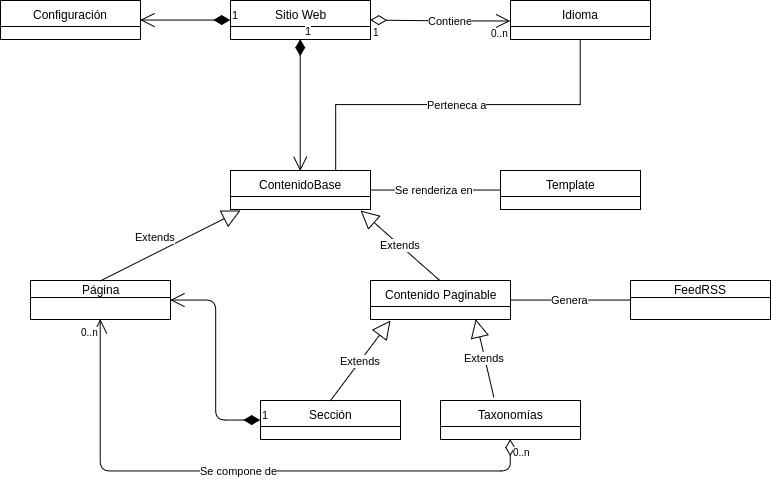
\includegraphics[width=1.1\textwidth]{4_analisis/modelo_conceptual}
    \caption{Modelo conceptual}
    \label{fig:modelo-conceptual}
\end{figure}

\subsection{Sitio web}

Representan el sitio web generado a partir de todos los contenidos que lo componen.

Relaciones:
\begin{itemize}
    \item Esta compuesto por varios contenidos.
    \item Está compuesto por una configuración.
\end{itemize}

\subsection{Configuración}

Representan la configuración básica del sitio.

Relaciones:
\begin{itemize}
    \item Pertenece a un sitio web.
\end{itemize}

\subsection{Idioma}

Representa a los idiomas disponibles en sitio.

Relaciones:
\begin{itemize}
    \item Pertenece a un sitio web.
\end{itemize}

\subsection{Contenido base}

Representa cualquier contenido que existe en un sitio.

Relaciones:
\begin{itemize}
    \item Pertenece a un sitio web.
    \item Se relaciona con una template en la que se tiene que renderizar.
    \item Se relaciona con un idioma.
\end{itemize}

\subsection{Contenido paginable}

Representa a un contenido, que a su vez está compuesto por otros contenidos, lo que implica
que es paginable.

Relaciones:
\begin{itemize}
    \item Extiende un contenido base.
\end{itemize}

\subsection{Página}

Representa la página que redacta un usuario.

Relaciones:
\begin{itemize}
    \item Extiende un contenido base.
    \item Pertenece a una sección.
    \item Se clasifica en varias taxonomías.
\end{itemize}

\subsection{Sección}

Representa a un conjunto de contenidos.

Relaciones:
\begin{itemize}
    \item Está compuesto por varias páginas.
    \item Extiende un contenido base.
\end{itemize}

\subsection{Taxonomías}

Representa la clasificación de contenidos.

Relaciones:
\begin{itemize}
    \item Extiende un contenido base.
    \item Contiene varias páginas.
\end{itemize}

\subsection{Template}

Representa la template HTML en la que se renderiza un contenido

Relaciones:
\begin{itemize}
    \item Se relaciona con un contenido.
\end{itemize}

\subsection{Feed RSS}

Representa la representación RSS de un contenido paginable

Relaciones:
\begin{itemize}
    \item Pertenece a un contenido paginable.
\end{itemize}

%%%%%%%%%%%%%%%%%%%%%%%%%%%%%%%%%%%%%%%%%%%%%%%%%%%%%%
%%%%%%%%%%%%%%%%%%%%%%%%%%%%%%%%%%%%%%%%%%%%%%%%%%%%%%

\section{Modelo de casos de uso}

El modelo de casos de uso representa las interacciones entre los actores y el sistema, 
desarrollado a partir de los requisitos descritos anteriormente.

\subsubsection{Actores}

En este apartado se describen los diversos roles que juegan los usuarios del sistema.
Para ese caso en concreto, sólo existirá un usuario ya que es el propio usuario
el que realiza todas las acciones para la generación de los contenidos.

\begin{figure}[h]
    \centering
    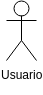
\includegraphics[width=0.1\textwidth]{4_analisis/actor}
    \caption{Diagrama de actores}
    \label{fig:actores}
\end{figure}

\subsubsection{Caso de uso: configuración del sitio}

\begin{description}
    \item[Descripción] El usuario debe de poder configurar todas las opciones disponibles
        a través de un fichero general de configuración
    \item[Actores] \textit{Usuario}.
    \item[Escenario principal] $\quad$
        \begin{enumerate}
            \item El \textit{Usuario} escribe el contenido del fichero de configuración.
            \item El \textit{Usuario} ejecuta la ejecución de contenido.
            \item El sitio se genera satisfactoria siguiendo todo los parámetros configurados.
        \end{enumerate}
    \item[Flujo alternativo] $\quad$
        \begin{description}
            \item[3a] Existe algún error de formato en el fichero y el sistema avisa al usuario.
        \end{description}
\end{description}

\subsubsection{Caso de uso: creación de contenidos}

\begin{description}
    \item[Descripción] El usuario debe de poder definir contenidos y generarlos en HTML.
    \item[Actores] \textit{Usuario}.
    \item[Escenario principal] $\quad$
        \begin{enumerate}
            \item El \textit{Usuario} define contenidos en la carpeta de contenidos.
            \item El \textit{Usuario} ejecuta la generación del sitio.
            \item El contenido de los ficheros es generado correctamente en HTML
        \end{enumerate}
    \item[Flujo alternativo] $\quad$
        \begin{description}
            \item[2a] El formato de alguno de los ficheros no es correcto y el sistema informa al usuario.
        \end{description}
\end{description}

\subsubsection{Caso de uso: metadatos de contenidos}

\begin{description}
    \item[Descripción] El usuario debe de poder definir metadatos en los ficheros, al inicio.
    \item[Actores] \textit{Usuario}.
    \item[Escenario principal] $\quad$
        \begin{enumerate}
            \item El usuario añade al inicio del fichero metadatos que necesita en la renderización de éstos.
            \item El usuario ejecuta la generación del sitio.
            \item El usuario puede usar esos metadatos al renderizar los contenidos en la templates.
        \end{enumerate}
    \item[Flujo alternativo] $\quad$
        \begin{description}
            \item[2a] Los metadatos no siguen el formato correcto y el sistema notifica al usuario.
        \end{description}
\end{description}

\subsubsection{Caso de uso: clasificación de contenidos}

\begin{description}
    \item[Descripción] El usuario debe de poder definir taxonomías y poder usarlas en los ficheros
    \item[Actores] \textit{Usuario}.
    \item[Escenario principal] $\quad$
        \begin{enumerate}
            \item El usuario define las taxonomías necesarias en el fichero de configuración.
            \item El usuario usa las taxonomías en los metadatos de los ficheros para clasificarlos.
            \item El usuario ejecuta la generación del sitio.
            \item Se generan tantas urls como taxonomías definidas con los contenidos asociados.
        \end{enumerate}
    \item[Flujo alternativo] $\quad$
        \begin{description}
            \item[3a] Se produce algún error en la generación y el sistema avisa al usuario.
        \end{description}
\end{description}

\subsubsection{Caso de uso: internacionalicación}

\begin{description}
    \item[Descripción] El usuario debe de poder definir más de un idioma.
    \item[Actores] \textit{Usuario}.
    \item[Escenario principal] $\quad$
        \begin{enumerate}
            \item El \textit{Usuario} define los idiomas deseados en la configuración.
            \item El \textit{Usuario} define contenido en todos esos idiomas.
            \item El \textit{Usuario} genera el sitio.
            \item El sitio se genera con cada contenido definido en el idioma que le corresponde
        \end{enumerate}
    \item[Flujo alternativo] $\quad$
        \begin{description}
            \item[3a] Existe algún problema en alguna de las configuraciones, el sistema avisa del error
                y cancela la ejecución.
        \end{description}
\end{description}

\subsubsection{Caso de uso: definición de plantillas}

\begin{description}
    \item[Descripción] El usuario debe de poder definir plantillas HTML en función del tipo de contenido.
    \item[Actores] \textit{Usuario}.
    \item[Escenario principal] $\quad$
        \begin{enumerate}
            \item El \textit{Usuario} define distintas templates en función del tipo de contenido.
            \item El \textit{Usuario} genera el sitio.
            \item El sitio renderiza correctamente los contenidos en las templates correspondientes.
        \end{enumerate}
    \item[Flujo alternativo] $\quad$
        \begin{description}
            \item[3a] Existe algún problema en la generación y el sistema avisa del error
                y cancela la ejecución.
        \end{description}
\end{description}

\begin{figure}[h]
    \centering
    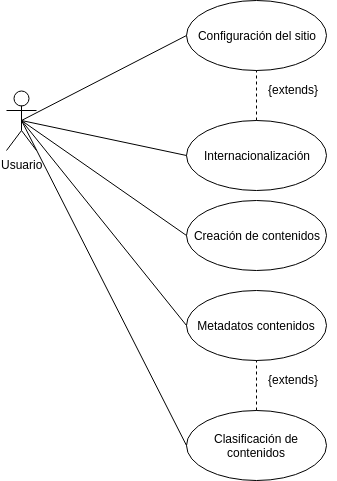
\includegraphics[width=0.7\textwidth]{4_analisis/casos_de_uso}
    \caption{Casos de uso}
    \label{fig:actores}
\end{figure}

%%%%%%%%%%%%%%%%%%%%%%%%%%%%%%%%%%%%%%%%%%%%%%%%%%%%%%
%%%%%%%%%%%%%%%%%%%%%%%%%%%%%%%%%%%%%%%%%%%%%%%%%%%%%%

% \section{Modelo de interfaz de usuario}
